
\chapter{Implementation}

This section describes the implementation of social network site
and how the system scales.

The system is composed by the following components, as shown in figure \ref{fig:system_architecture}: At the first layer lives (1) the Social Networking engine, which runs all PHP scripts and described in section \ref{sec:implementaion_of_social_netowrk}. At the second layer lives (2) the Memcached caching system, which described in section \ref{sec:memcache_implementation}. At the third layer lives (3) the Social Network MySQL database, and (4) the CDO server - client components and the CDO repository.

\begin{figure}[h]
	\caption{The overall architecture of Social Network.}
	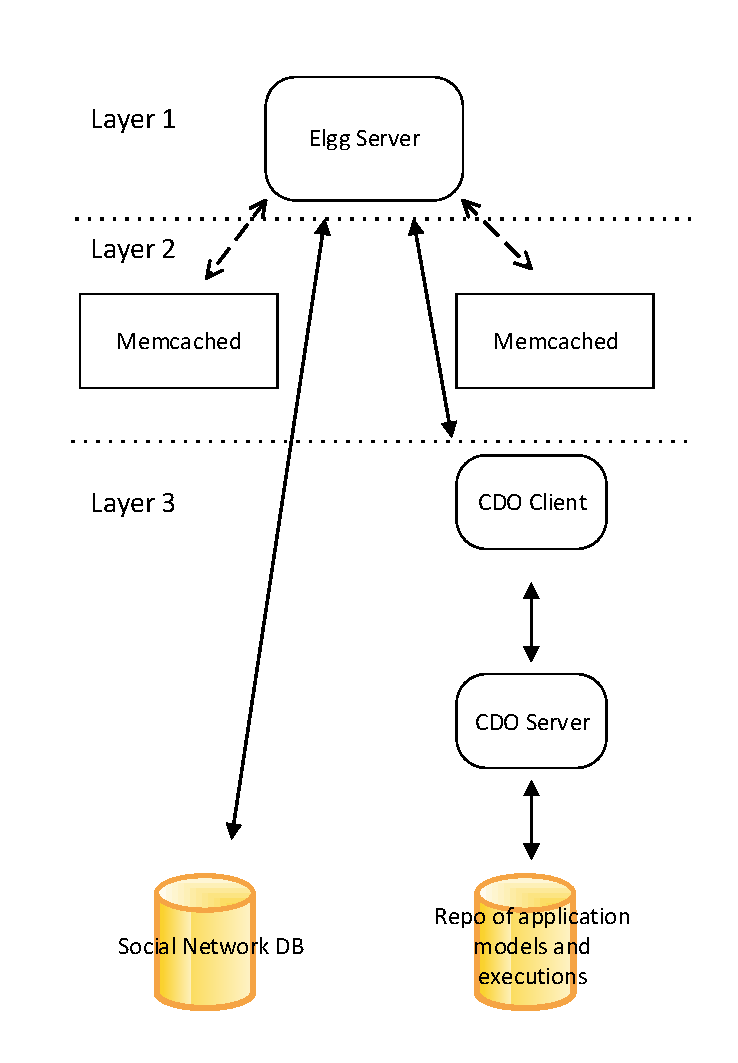
\includegraphics[width=0.6\textwidth,natwidth=200,natheight=150]{./fig/system_architecture.pdf}
	\centering
	\label{fig:system_architecture}
\end{figure}

Achieving the scalability of the system, two system architectures are examined at two layers of the system: (1) We added more than one Social Network engine at the first layer of the system. In this implementation, in order to keep the file system in consistent mode we integraded Apache Zookeeper\cite{zookeeper_url}. (2) We added more than one memcached machines at the second layer in order to add more cpu capacity and improve the system response time.

\section{Implementation of Social Network}
\label{sec:implementaion_of_social_netowrk}
The social networking platform is implemented over the extensible Elgg social network framework\cite{elgg_url}.  Elgg is open source software written in PHP, uses MySQL for data persistence and supports jQuery~\cite{jquery_url} for client-side scripting.  The architecture of Elgg Social Network shown in figure ~\ref{fig:elgg_architecture}. The Model of the framework is structured around the following key concepts as shown in figure ~\ref{fig:elgg_entities}:
\begin{itemize}
\item \emph{Entities}, classes capturing social networking concepts: users, communities, application models. Elgg Core comes with four basic objects: ElggObject, ElggUser, ElggGroup, ElggSite, ElggSession, ElggCache and a lot of other classes necessary for the proper engine operation.
\item \emph{Metadata} describing and extending entities (e.g., a response to a question, a review of an application model, etc.).
\item  \emph{Relationships} connect two entities (e.g., user A is a friend of user B, user C is a contributor to an application model, etc.) and are persisted in the Social Network DB.
\item \emph{Annotations} are pieces of simple data attached to an entity that allow users to leave ratings, or other relevant feedback.
\end{itemize}
All Elgg objects inherit from ElggEntity, which provides the general attributes of an object. Elgg core comes with the following basic entities: ElggObject, ElggUser, ElggGroup, ElggSite, ElggSession, ElggCache, as well as other classes necessary for the operation of the engine.

\begin{figure}[h]
	\caption{The Elgg Engine Data model.}
	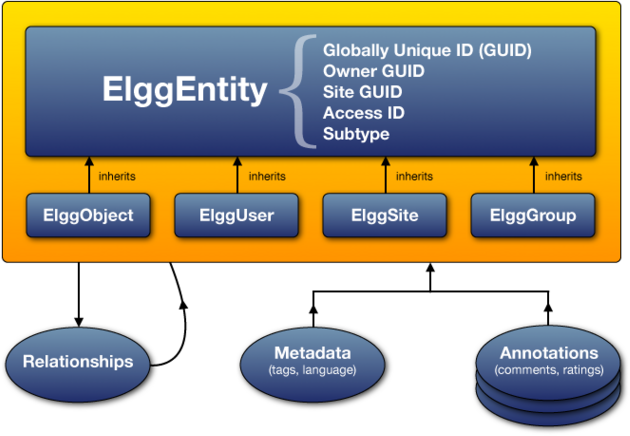
\includegraphics[width=0.6\textwidth,natwidth=200,natheight=150]{./fig/elgg_data_model.png}
	\centering
	\label{fig:elgg_entities}
\end{figure}

Elgg comprises a core system that can be extended through plugins (examples are the Cart system or the handling of Application Models). Plugins add new functionality, can customize aspects of the Elgg engine, or change the representation of pages.
A plugin can create new objects (e.g., ApplicationObject) characterized (through inheritance of ElggEntity) by a numeric globally unique identifier (GUID), owner GUID, Access ID. Access ID encodes permissions ensuring that when a page requests data it does not touch data the current user does not have permissions on. 

Figure\ref{fig:elgg_architecture} shows the model, view, and control parts of Elgg's architecture. In a typical scenario, a web client requests an HTML page (e.g., the description of an application model).  The request arrives at the \emph{Controller}, which confirms that the application exists and instructs \emph{Model} to increase the view counter on the application model object. The controller dispatches the request to the appropriate handler (e.g., application model, component handler, community handler) which then turns the request to the view system. View pulls the information about the application model and creates the HTML page returned to the web client.


\begin{figure}[h]
	\caption{Architecture of the Elgg Social Networking engine.}
	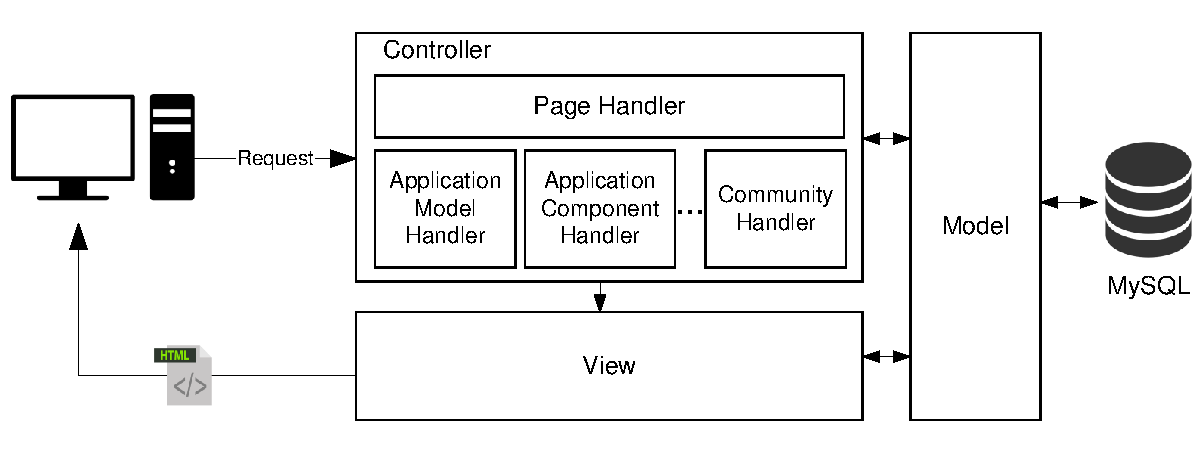
\includegraphics[width=0.6\textwidth,natwidth=200,natheight=150]{./fig/elgg_architecture.pdf}
	\centering
	\label{fig:elgg_architecture}
\end{figure}


The extensibility of Elgg can be established not by modifying the core system but by introducing new plug-ins which follow the MVC model. A new plug-in can create a new entity. Thus, each entity is characterized by a numeric Globally Unique Identifier and Access ID. The Access ID determines the permissions that other users have. Thus, when a page requests data, it never touches those data that the current user does not have permission to see. All plug-ins share a common structure of folders and PHP files, following the MVC model of figure~\ref{fig:elgg_architecture}. 

The hierarchy of a plug-in is shown in figure~\ref{fig:elgg_hierarchy}. 
Folder {\em actions} includes the actions applied on application models. Every active participation by the user is performed via an action. Logging in, creating, updating or deleting content are all generic categories of actions.
The {\em views} folder contains the {\em php} forms applied on application models, {\em river} events (Elgg terminology for live feeds). Viewss are responsible for creating the output for the client browser. Generally, this will be HTML, but it can be also JSON or other format. 
{\em Pages} overrides elements of core Elgg pages and can be from chunks of presentation output (like sidebars) down to individual html code.  
The {\em js} and {\em lib} folder provides javascript and {\em php} library functions. 
Finally, the {\em vendors} folders include third-party frameworks such as Twitter's bootstrap front-end~\cite{bootstrap_url}.
The most important file of a plug-in is the \emph{start.php} script, which contains the \emph{page handler}. Page handler is a function manages the plug-in pages enabling custom url redirect to a specific page. 
The plug-in initialization is also defined in the start.php and registers actions, events and determines the views. 

\begin{figure}[h]
	\caption{The structure of the application description plug-in.}
	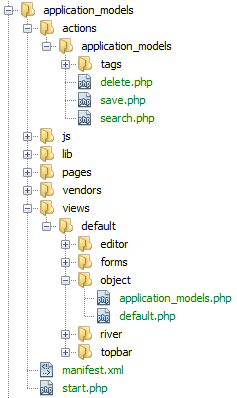
\includegraphics[width=0.4\textwidth]{./fig/folder_hierarchy.png}
	\centering
	\label{fig:elgg_hierarchy}
\end{figure}

The execution history of deployments of application models and the description of those models is stored in the CAMEL information repository, which is implemented as an Eclipse CDO server. The exchange of information between Elgg and the CAMEL information repository is going through CDO Client who retrieves the information from CDO server and sent it to the Elgg over sockets.

\subsection{Scaling Social Network Engine}
\label{sec:engine_scale}

This subsection describes how the horizontal scale of Social Network engine achieved. At the layer 1 of figure~\ref{fig:elgg_architecture} lives the Apache2 server which as the stress test of the system shows in chapter~\ref{chapt:evaluation}, the Apache2 server takes a heavy load on CPU utilization. Therefore, we introduce more than one Apache2 Servers running the Social Networking Engine of Elgg Framework. 

The Social Networking Engine keeps some information in the file system instead of the Social Network DB. This information includes the profile photos of users and any other photo such as photos that users add to the community groups. Furthermore, the initial configuration of Social Networking Engine keeps in the file system some caching files representing some views which are independent from specific users and do not change among all users. This file system caching feature removed from the Social Network Engine because is more efficient to use memcached for the caching instead of the slow file system.

The Network File System (NFS) is used in order to all SN Engines have access to the same file system store. An NFS server installed in one of the SN Engines and all the other SN Engines have an NFS client accessing the remote file system.   

Distributing Social Network Engine was not an easy problem, so Apache ZooKeeper~\cite{zookeeper_url} is used to enable highly reliable distributed coordination among access to the file system storing by Social Networking Engine. 
Apache ZooKeeper provides a tree abstraction where every node in that tree (or znode) is a file on which a variety of simple operations can be performed. ZooKeeper orders operations on znodes so that they occur atomically. Therefore there is no need to use complex locking protocols to ensure that only one process can access a znode at a time. The tree represents a hierarchical namespace, so that many distinct distributed systems can use a single ZooKeeper instance without worrying about their files having the same name.

Social Networking Engine uses Apache ZooKeeper in order to keep consistent the file system in rear but possible scenarios such as two users try to upload in the same time a file to the same group. When a SN Engine wants to write a file in file system first locks the specific path and after finish the write operation releases the lock.


\section{User interface}
The design of User interface of Social Network based on 102 mock-ups designed by HCI experts. In order to support those look \& feel and the functionality of those mock-ups 25K lines of php, js and css code is written. \ldots

\section{Memcache}
\label{sec:memcache_implementation}
This section describes the experience gained by using memcached\cite{memcache_url}. Memcached is an open source, high-performance, distributed memory object caching system. We choose memcached, because is a generic simple in-memory key-value store. It has a powerful API available for PHP. After memcached integration the system increase the response time and performance.

Memcached added in layer 2 of system architecture and used for storing the following key-value tuples: (1) values from Social Network Database such as entities of Social Network, applications, components, users, group discussions, (2) evaluated javascript code results and (3) executions histories from repository of application models. Storing the executions of applications at Memcached the response time of the system increased because the PHP modules do not need to go through the heavy CDO client but get directly the executions of applications from Memcached.

The apache jmeter\cite{jmeter_url} was used to measure the responce time of the system and the sysstat tool\cite{sysstat_url} was used to measure the cpu usage. Section \ref{sec:eval_memcache} 
 shows the performance results of this implementation.

All tuples at Memcached are inserted with maximum key expiration time of thirty days. When a value in social network is updated, the memcached key will deleted~\ref{fig:memcache_key_value}.

\begin{figure}[h]
	\caption{The scenario a depicts a request from memcached when the key does not exist and scenario b depicts a updated operation of a value) }
	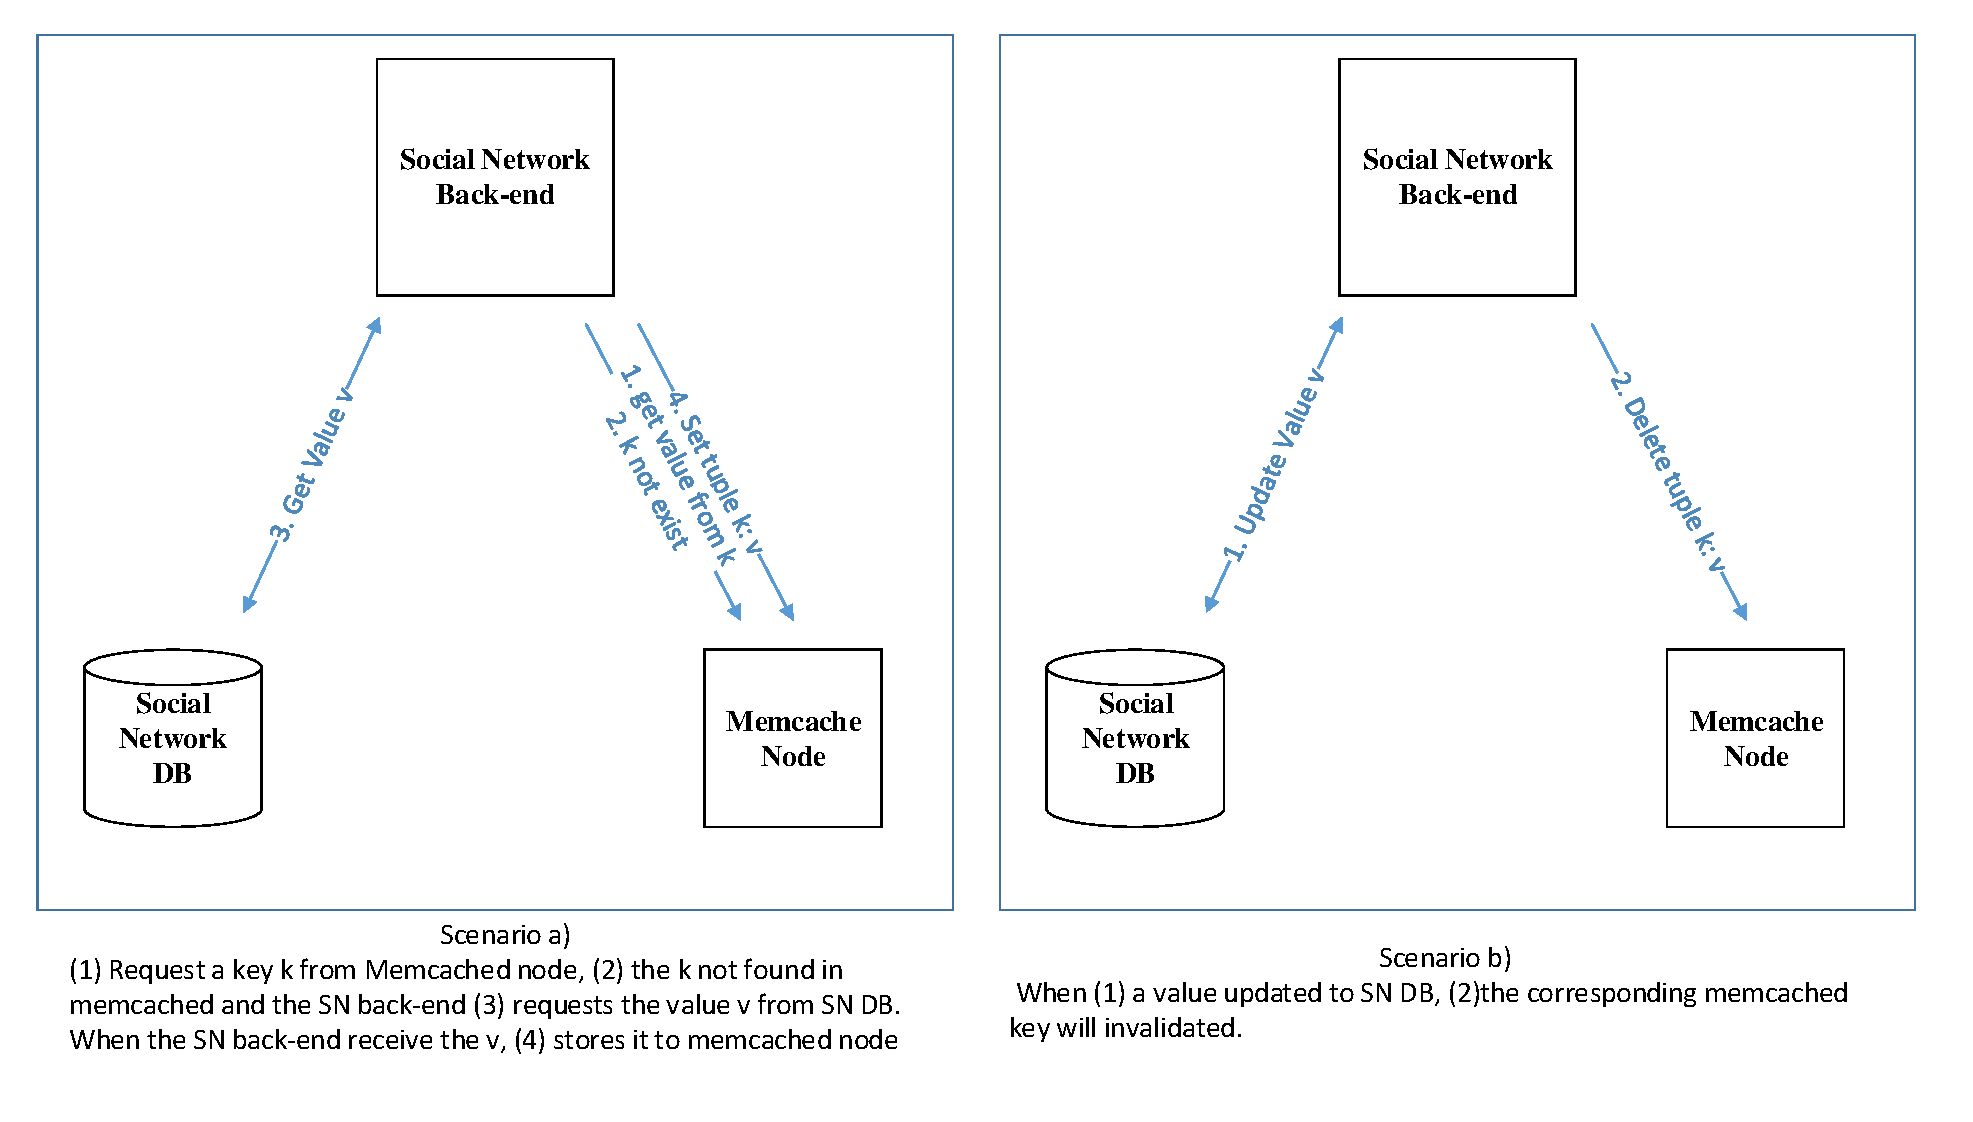
\includegraphics[width=0.9\textwidth]{./fig/memcached_key_value.pdf}
	\centering
	\label{fig:memcache_key_value}
\end{figure}

\section{Natural Language Processing}
Natural Language Processing(NLP)~\cite{manning1999foundations} is feature added to Social Network. NLP concerned with the interactions between the users of SN and how the platform can understand and determine the type of user input. Particularly, Natural Language Understanding using Naivy Bayes algorithm is added to SN. The Natural framework~\cite{nodenatural_url} implemented with node.js is used. In general, Machine Learning algorithms such as Naivy Bayes, wants an input data set of training data. Those data is pooled from StackOverflow. When users ask questions in StackOverflow, must specify tags describing their questions. Those questions is an excellent repository to train the NB algorithm. NB is trained with 50K questions from StackOverflow Q\&A site, fifty questions for each tag. The general algorithm is shown below. First, the algorithm starts with a tag which is relevant to the Social Network Platform such as \emph{scalability} at line 01. Afterwards, using the stackexchange api the algorithm gets the 50 most voted questions tagged with \emph{scalability}. For each question (line 04), the trainClassifier clears the body from html tags inserted by the StackOverflow users to beatify their questions (line 05) and classify this question's body with each tag. Automatically, the trainClassifier proceeds to the next tag of this question. When the trainClassifier is finished the NB is trained with 50K questions, fifty questions per tag. It should be noted that a question may have more than one tag, so a question maybe classified up to five tags / classes.

\begin{lstlisting} 
01:var tags = ['scalability']
02:trainClassifier(0)
03:function trainClassifier(index) {
04:  var questions = stackexchange.api.getQuestionsByTag(tags[index])
05:  foreach(questions as q)
06:    body = clear(q.body)
07:    foreach(q.tags as t)
08:    	 classify(body, t)
09:    	 if(not tags.exist(t) and tags.length() < threshold)
10:    	   tags.push(t)	  
11:        trainClassifier(tags.indexOf(t))
12:}		
\end{lstlisting}